\cotefile{136}
\scanpage{362}\mspage{1}
\uuline{Formule de Decalage} (Quillen - Bousfield) [cf \unsure{thèse|Thèse} Illusie].

\[
\deleted{\unsure{F|H}}\qquad L_{*}F(M,n)\qquad L_{*}F(M[n])
\]
\[
\begin{aligned}
&\deleted{L_i\operatorname{Sym}^{j}(M,n)\simeq L_{i+n}\Lambda^{j}(M,n+1)}\\
&\deleted{L_i\Lambda^{j}(M,n)\simeq L_{i+n}\Gamma^{j}(M,n+1)}
\end{aligned}
\]
\margin{$\underline M\longrightarrow\underline M$}
\[
\deleted{\unsure{L_i\Gamma^{j}(M,n)}\simeq\unsure{L_{i+n}\Lambda^{j}}}
\]
\diagram{\begin{tikzcd}[ampersand replacement=\&]
K(M,n)\arrow[r] \& E(M,n+1)\arrow[d,dash]\\
\& K(M,n+1)
\end{tikzcd}}
\[
\begin{aligned}
&\operatorname{Sym} K(M,n)\otimes\Lambda E(M,n+1).\\
&\hspace{7em}\Lambda^{n+1}\Phi\otimes_{\mathbb Z}M
\end{aligned}
\]

{\scriptsize
\[
\begin{aligned}
0&\longrightarrow\operatorname{Sym}^{i}K(M,n)\longrightarrow
\operatorname{Sym}^{i-1}K(M,n)\otimes\underline{\Lambda^{1}E(M,n+1)}
\longrightarrow\operatorname{Sym}^{i-2}K(M,n)\otimes\underline{\Lambda^{2}E}(M,n+1)\\
&\hspace{14em}\longrightarrow\Lambda^{i}E(M,n+1)\longrightarrow\Lambda^{i}K(M,n+1)\longrightarrow0
\end{aligned}
\]
\[
\begin{aligned}
0&\longrightarrow\Lambda^{i}K(M,n)\longrightarrow\Lambda^{i-1}K(M,n)\otimes\operatorname{Sym}^{1}E(M,n+1)
\longrightarrow\cdots\operatorname{Sym}^{i}E(M,n+1)\\[-1pt]
0&\longrightarrow\Gamma^{i}K(M,n)\longrightarrow\Gamma^{i-1}K(M,n)\otimes\Lambda^{1}E(\cdots)
\end{aligned}
\]
}
\begin{flushright}
$\searrow\ \operatorname{Sym}^{i}K(M,n+1)\searrow 0$
\end{flushright}
\[
\boxed{\underline{L_r\operatorname{Sym}^{i}K(M,n+1)}\simeq L_{r-i}\Lambda^{i}K(M,n)}
\]
\[
\begin{aligned}
L_{*}\operatorname{Sym}^{i}X[1]&\simeq L_{\unsure{*-i|*}}\Lambda^{i}X[-i]\\
L_{*}\Lambda^{i}(X[1])&\simeq L_{*}\Gamma^{i}X[-i]\\
L_{*}\operatorname{Sym}^{i}X[2]&\simeq L_{*}\Gamma^{i}X[-2i]
\end{aligned}
\]
\noindent $-$
% archive sheet number: 363
\scanpage{363}\mspage{2}
\uline{(Th) Dold Puppe} Ann Inst Fourier.
\[
L_r\operatorname{Sym}_{\unsure{z|\mathbb Z|e}}^{*}\simeq L_r\mathbb Z[\qquad]
\]
\[
\Gamma\qquad M_{\bullet}\ \text{un \inserted{complexe de chaines de} $A$-modules}
\]
\margin{du moins pour $M$ concentré en un seul degré}
\[
\deleted{K(M_{\bullet})}
\]
\[
\begin{aligned}
\text{Def}\quad & L_{\unsure{i|r}}\mathbb Z M_{*}=H_i(M_{*})\\
&\quad\unsure{\wr\wr|\rotatebox{-90}{$\supseteq$}}\\
& L_i\bigl(\operatorname{Sym}(M_{*})\bigr)
\end{aligned}
\]
\margin{D'où une graduation (dite la graduation par le poids sur l'homologie des esp d'E.M).}

\uline{Pt clef} : Th de Dold-Thom :
\[
\begin{aligned}
X\quad&\text{un espace} &\operatorname{SYM}^{\infty}X\\
&&\unsure{*|\cdot}\ \cup X\cup X^{(2)}\cup X^{(3)}\ldots
\end{aligned}
\]
\[
X\longrightarrow
\tikz[baseline=(a.base)]{\node[inner sep=1pt](a){$\pi_i\operatorname{SYM}^{\infty}X$};\draw (a.center) ellipse (1.35cm and .34cm);}
\simeq H_i X
\qquad
\begin{aligned}&\mathbb Z X\\&\pi_i\underline{\mathbb Z X}\end{aligned}
\]
Satisfait \deleted{\unsure{à}} \inserted{aux axiomes} Eilenberg-Steenrod

\begin{center}\rule{1.7cm}{0.35pt}\end{center}
\margin{$G=\mathbb Z^{k}\unsure{\times|+}\mathbb Z$}
\[
X\quad\text{un espace de Moore}\quad
\tikz[baseline=(a.base)]{\node(a){$\mathbb Z M(G,n)$};\draw(a.center) ellipse (1.25cm and .36cm);}. \qquad G
\]
\[
K(G,n)\sim
\tikz[baseline=(a.base)]{\node(a){$\operatorname{Sym}^{\infty}M(G,n)$};\draw(a.center) ellipse (1.55cm and .35cm);}
\]
\diagram{\begin{tikzcd}[ampersand replacement=\&,column sep=small,row sep=small]
H_i(G,n)=\pi_i\mathbb Z K(G,n)\arrow[r,phantom,"\overset{\text{Dold Thom}}{=}"] \&
\pi_i\mathbb Z\operatorname{Sym}^{\infty}M(G,n)\\
\&\pi_i\operatorname{Sym}(\underline{\mathbb Z M(G,n)})\arrow[u,"\sim"']\\
\&=L_i\operatorname{Sym}(G)\quad\deleted{\unsure{K(G,n)}}
\end{tikzcd}}
\margin{$G\longrightarrow M(G)$}
\[
\deleted{\unsure{M(G),M(H)}\longrightarrow\unsure{\operatorname{Hom}(G,H)}}
\]
Theoreme de Dold.
\[
\mathbb Z\operatorname{Sym}^{\infty}X\overset{\sim}{\longleftarrow}\operatorname{Sym}\underline{\mathbb Z X}
\]
\[
\deleted{\unsure{\operatorname{Ext}(G,H)}}
\]
\deleted{\unsure{Fonc|Free}} Par def
\[
\mathbb Z M(G,n)\sim K(G,n)
\]
\[
\begin{aligned}
H_{n+r}K(M,n)&\overset{S}{\simeq} H_{n+r+1}K(M,n+1)\\
&\deleted{\unsure{n\leq r<2n|n\leq r\leq 2n}}\\
&r<n .
\end{aligned}
\]
% archive sheet number: 364
\scanpage{364}\mspage{3}
\[
\underline{H_{*}(K(\mathbb F_p,n),\mathbb F_p)}^{*}
\simeq H^{\deleted{\unsure{*}}n+r}(K(\mathbb F_p,n),\mathbb F_p)
\]
\[
K(\mathbb Z,\unsure{n|1})\longrightarrow K(\mathbb Z,n)\longrightarrow K(\mathbb F_p,n)
\]

Puisque $K(\mathbb F_p,n)$ represente la $\mathbb F_p$, coh
\[
(\mathbb F_p,n,\mathbb F_p,n+r)
\qquad r<n
\]
\margin{$\downarrow$ operations coh de type}

Operations stables de deg $r$\quad $\{P_{r}\}$\quad Une collection $\forall n$
\[
H^n(X,\mathbb F_p)\longrightarrow H^{n+r}(X,\mathbb F_p)
\]
commute
\diagram{\begin{tikzcd}[ampersand replacement=\&,row sep=small]
\bar H^{n+1}(SX,\mathbb F_p)\arrow[r,"P_{n+1}"]\arrow[d,phantom,"\rotatebox{90}{$\approx$}"] \&
\bar H^{n+1+r}(SX,\mathbb F_p)\arrow[d,phantom,"\rotatebox{90}{$\approx$}"]\\
\widetilde H^n(X,\mathbb F_p)\arrow[r,"P_n"] \& \widetilde H^{n+r}(X,\mathbb F_p)
\end{tikzcd}}
\margin{$r<n$}
\diagram{\begin{tikzcd}[ampersand replacement=\&,row sep=small,column sep=tiny]
\& H^{n+r}(K(\mathbb F_p,n),\mathbb F_p)\arrow[dl]\arrow[r,phantom,"\simeq"] \&
H^{n+r+1}(K(\mathbb F_p,n+1),\mathbb F_p)\\
H^{n+r-1}(K(\mathbb F_p,n-1),\mathbb F_p)\& P_n^{\prime}\& P_{n+1}^{\prime}
\end{tikzcd}}

\uuline{Operations stables} : Les op stables sont \deleted{\unsure{d}} données par l'algebre de Steenrod
\[
\begin{aligned}
p&\ne2\\
&\mathbb F_p\underline{[P^0,P^1,\ldots P^n,\ldots,\beta]}\\
&P^0=1\qquad\deg P^i=2i(p-1)\qquad\deg\beta=1
\end{aligned}
\]
Relations d'Adem

\noindent Cohomology operations\\
Steenrod + Epstein\\
Ann of Math Studies N\textsuperscript{o} 50\\
Princeton\\
p 77
% archive sheet number: 365
\scanpage{365}\mspage{4}
$P^i$ op stables construites par Steenrod.

\[
\begin{aligned}
p=2\qquad &\underline{\mathbb F_2[\operatorname{Sq}^{i}]} & i\geq0\\
\deg\operatorname{Sq}^{i}=i\qquad&
\operatorname{Sq}^{0}=1\qquad(\operatorname{Sq}^{1}=\beta)&\text{rel d'Adem}
\end{aligned}
\]
\[
\begin{aligned}
&\hspace{13em}p\ 2\\
&\deleted{\operatorname{Sq}^{1}\operatorname{Sq}^{2}=\operatorname{Sq}}\qquad
\operatorname{Sq}^{1}\operatorname{Sq}^{2}=\operatorname{Sq}^{3}+\operatorname{Sq}^{2}\operatorname{Sq}^{1}\qquad(?)\\
&\hspace{13em}\text{etc}\ \ldots
\end{aligned}
\]
\begin{center}\rule{1.3cm}{0.3pt}\end{center}
Formule de Cartan :
\[
P^i(x\times y)=\sum_{j\geq0}P^j(x)P^{i-j}(y)
\]
\[
\begin{aligned}
P^I&=\beta^{\varepsilon_0}P^{\eta_1}\beta^{\varepsilon_1}P^{\eta_2}\ldots
& I&\unsure{=|\sim}(\varepsilon_0,\eta_1,\varepsilon_1,\eta_{\unsure{i|2}},\ldots)\\
&& \varepsilon_i&=0,1\\
&& \eta_i&\geq0
\end{aligned}
\]
$\deg I$ de maniere evidente

\unsure{excès|exces} $e(I)=\text{``}\eta_1-\sum_{i>1}\eta_i\text{''}$

admissible
\[
\eta_i\geq p\eta_{i+1}+\varepsilon_i
\]
les $P^I$ admissibles forment une $\mathbb F_p$-base .

\begin{center}\rule{1.8cm}{0.3pt}\end{center}
\diagram{\begin{tikzcd}[ampersand replacement=\&,row sep=tiny]
|[draw,circle]| A\arrow[r] \& H^{*}(K(\mathbb F_p,n),\mathbb F_p)\\
x\&x\,\iota_n
\end{tikzcd}}
\uline{Theoréme} : \margin{Serre ($p=2$)}
$H^{*}(K(\mathbb F_p,n),\mathbb F_p)={}$ Algebre anticommutative libre sur $\mathbb F_p$ engendrée par les \uline{\unsure{monomes|monoms} admissibles} d'exces $<n$.

$H_{*}(\underline{K(\mathbb F_p,n)},\mathbb F_p)={}$ Alg anticom à puiss divisée universelle engendrée par les elements duaux.
% archive sheet number: 366
\scanpage{366}\mspage{5}
\uline{Dem 1)} Seminaire Cartan

On regarde la suite spectrale du classifiant
\[
E_2=\operatorname{Tor}^{H_{*}(K(\mathbb F_p,n),\mathbb F_p)}
(\mathbb F_p,\mathbb F_p)\Longrightarrow H_{*}(\underbrace{K(\mathbb F_p,n+1)}_{\displaystyle =B_{K(\mathbb F_p,n)}},\mathbb F_p]
\]
Suite sp d'Eilenberg - Moore

Steenrod - \unsure{Rothenberger|Rollenberger|Rothenberg}, etc $\longrightarrow$
\diagram{\begin{tikzcd}[ampersand replacement=\&,column sep=small,row sep=tiny]
\cdots\& \mathbb Z(G\times G)\& |[draw,circle]| \mathbb Z G\arrow[r] \&\mathbb Z\\
\cdots\&\mathbb Z G\otimes\mathbb Z G\arrow[ur,shift left]\arrow[ur,shift right]\arrow[ur,shift right=2]\&\&
\end{tikzcd}}
\[
\deleted{\otimes\mathbb Z K(\mathbb F_p,\unsure{n|1})}
\qquad N\underline{\underline{\mathbb Z K(\mathbb F_p,n)}}=\underline M
\]
alg diff graduée augmentée.

Bar Constr
\diagram{\begin{tikzcd}[ampersand replacement=\&,column sep=small]
\cdots \& \deleted{\unsure{\otimes}}H_{*}(K(\mathbb F_p,n)^{\otimes 2}
\arrow[r,shift left]\arrow[r]\arrow[r,shift right]\&H_{*}K(\mathbb F_p,n)\arrow[r]\&M.
\end{tikzcd}}
\begin{center}\rule{2.2cm}{0.3pt}\end{center}
\[
\begin{aligned}
A=\mathbb Z(G)&\qquad\mathbb Z(EG)=*\\
&\tikz[baseline=(a.base)]{\node(a){$\mathbb Z(BG)$};\draw(a.center) ellipse (.85cm and .30cm);}
\end{aligned}
\]
\begin{center}\rule{3cm}{0.3pt}\end{center}

2) Methode de Serre \quad \unsure{Comm|Comn} Helv \qquad 1954

\margin{Springer : Symposium en l'honneur de Steenrod \inserted{Article de} May.}
\[
H^{*}(K(\mathbb F,n+1,),\mathbb F_p)\otimes
\underline{H^{*}(K(\mathbb F_p,n),\mathbb F_p)}\Longrightarrow\underline{H^{*}(*)}
\]
% archive sheet number: 367
\scanpage{367}
Comult naturelle sur $A$

$P$ operation coh
\[
(\mu^{*}P)(xy)=\sum P_i\unsure{{}'|{}}x\cdot P_{\unsure{j|i}}y
\]
Par la formule de Cartan
\[
\Delta P^i=\sum_{j+k=i}P^j\otimes P^k .
\]
\uline{Milnor} :
\[
\begin{aligned}
j\geq1\quad&\xi_{\text{\textcircled{$\scriptstyle j$}}}\quad\text{dual de}\quad
\underbrace{\underline P^{p^{j-1}}\ldots\underline P^{p^2}\underline P^{p}P^{p^0}}_{\text{monome adm}}\\
j\geq0\quad&\tau_j\qquad P^{p^j}\ldots P^p P\beta
\end{aligned}
\]
\[
\begin{aligned}
&\deleted{\unsure{H_{*}(K)}}\quad\underset{\text{dual de $A$}}{A_{*}}
=\operatorname{Sym}(\xi_i)\otimes\Lambda(\tau_{\deleted{k}j})\\
&\Delta\xi_k=\sum_i\xi_{k-i}^{p^i}\otimes\xi_i\\
&\Delta\tau_k=\tau_k\otimes1+\sum_{i=0}^{k}\xi_{k-i}^{p^i}\otimes\tau_i
\end{aligned}
\]
\margin{p 85}

\[
\begin{aligned}
L\operatorname{Sym}^{r}&=0\qquad r\ne p^s\quad s\geq0\\
L\operatorname{Sym}^{p^s}&K(\mathbb F_p,\unsure{n|m})\\
L_{n+i}\operatorname{Sym} K(\mathbb F_p,n)&
\xrightarrow[+1]{S}L_{n+i+1}\operatorname{Sym}K(\mathbb F_p,n+1)\\
L_{\unsure{*|x}}^{st}\tikz[baseline=(s.base)]{\node[draw,circle,inner sep=1pt](s){$\operatorname{Sym}$};}\mathbb F_p&=A_{*}\\
L_{*}^{st}\deleted{\unsure{\mathbb Z|\mathbb F_p}}\mathbb F_p[\mathbb F_p]&\unsure{=|\simeq}
\end{aligned}
\]
\[
\begin{aligned}
1+\operatorname{Sym}^{p^0}\qquad&\xi_1,\ \tau_0\qquad\in\operatorname{Sym}^{p}\\
&\xi
\end{aligned}
\]

\begin{center}\rule{.8\linewidth}{0.3pt}\end{center}
\[
A\otimes B\longrightarrow C\qquad \mathbb F_p\text{-modules}
\]
\[
K(A,i)\wedge K(B,j)\longrightarrow K(C,i+j)
\]
cup-products \unsure{pairings|pairengs}

Ce cup produit $K(\mathbb F_p,n)\wedge K(\mathbb F_p,m)\longrightarrow K(\mathbb F_p,m+n)$ induit en coh la comultiplication sur l'alg de Steenrod $A$ correspondant à la multiplication dans la duale
\[
\begin{aligned}
H^{*}(K(\mathbb F_p,n)\otimes H^{*}(K(\mathbb F_p,\unsure{n|m})
&\longleftarrow H^{*}(K(\mathbb F_p,m+n),\mathbb F_p)\\
A\otimes A&\longleftarrow A
\end{aligned}
\]
% archive sheet number: 368
\scanpage{368}
\[
A\xrightarrow{\varepsilon}\mathbb F_p
\]
\margin{$A$ $\mathbb F_p$ alg diff graduée aug sur $\mathbb F_p$}
\[
\begin{aligned} &B(A)\\ &\bar B(A):\end{aligned}
\]
\diagram{\begin{tikzcd}[ampersand replacement=\&,column sep=small]
\underline A\otimes A\otimes A\arrow[r,shift left=2]\arrow[r]\arrow[r,shift right=2]\&
\underline A\otimes A\arrow[r,shift left,"\mu"]\arrow[r,shift right,"1\otimes\varepsilon"']\&
A\arrow[l,bend right=55]\arrow[r]\&\mathbb Z EG
\end{tikzcd}}
\diagram{\begin{tikzcd}[ampersand replacement=\&,column sep=small,row sep=tiny,execute at end picture={\draw (current bounding box.center) ellipse (3.05cm and .65cm);}]
A\otimes A\arrow[r,shift left=2]\arrow[r]\arrow[r,shift right=2]\&
A\arrow[r,shift left]\arrow[r,shift right]\arrow[d,phantom,"\rotatebox{90}{$\in$}" description]\&
\deleted{\unsure{\mathbb Z}}\mathbb F_p\&\underline{\mathbb Z BG}\\
\&a\&\&
\end{tikzcd}}
\margin{$\underbrace{a\otimes\cdots\otimes a}_{n\ \mathrm{fois}}$}
$A$ commutative
\diagram{\begin{tikzcd}[ampersand replacement=\&,column sep=small,row sep=small]
{}\arrow[r,shift left=3]\arrow[r,shift left=1]\arrow[r,shift right=1]\arrow[r,shift right=3]\&
\mathbb Z G^3\arrow[r,shift left=2]\arrow[r]\arrow[r,shift right=2]\&
\underline{\mathbb Z G^2}\arrow[d,dash]\arrow[r,shift left]\arrow[r,shift right]\&
|[draw,circle]| \mathbb Z G\\
\&{}\arrow[r,shift left=2]\arrow[r]\arrow[r,shift right=2]\&
\mathbb Z G\otimes\mathbb Z G\arrow[ur,shift left]\arrow[ur,shift right]\&
\end{tikzcd}}
\margin{Bar \unsure{Constr|Consts} sur l'alg $\mathbb Z G$}

\[
A\otimes A.\qquad A\ \unsure{\longrightarrow|\text{---}}\unsure{\mathbb Z}
\]
\[
\begin{aligned}
A&=\mathbb Z K(G,n)\\
\bar B(A)&\sim\mathbb Z B K(G,n)
\end{aligned}
\]
Structure d'algebre de $\bar B(A)$

E zilber
\margin{$A$ comm $\Rightarrow$ $I\otimes A\otimes A\longrightarrow A$ hom d'alg}
\diagram{\begin{tikzcd}[ampersand replacement=\&,column sep=small]
\bar B(A)\otimes\bar B(A)\arrow[r,shift left]\&
\bar B(A\otimes A)\arrow[l,shift left]\arrow[r]\&\bar B(A)
\end{tikzcd}}
% archive sheet number: 369
\scanpage{369}
% printed form
% Blank ruled face. The isolated dark strokes at the right show through the
% perforations of this leaf. The archive number is below the last ruling.
\figure{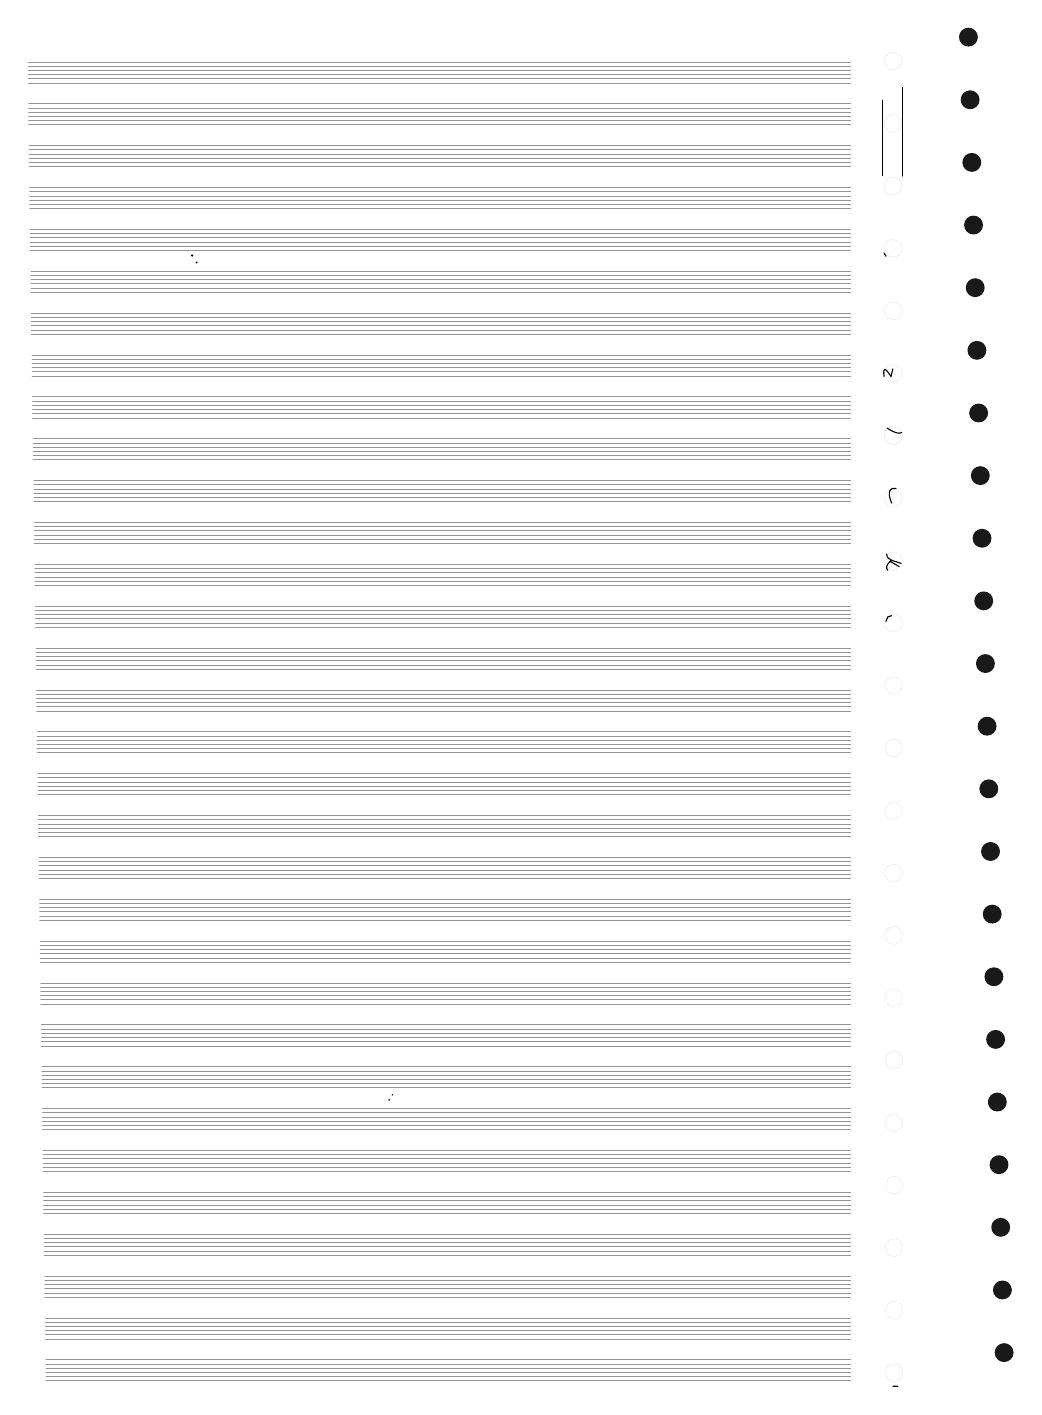
\begin{tikzpicture}[x=.008cm,y=-.008cm,line cap=round]
\foreach \g in {0,...,31}{
  \foreach \h in {0,1,2,3,4,5}{
    \draw[black!42,line width=.12pt] ({18+0.92*\g},{105+66.5*\g+6.7*\h})
      -- (1325,{105+66.5*\g+6.7*\h});
  }
}
\foreach \h in {0,...,21}{\draw[black!10,line width=.16pt]
({1392+.10*\h},{104+99.2*\h}) circle[radius=14];}
\foreach \h in {0,...,21}{\fill[black!90] ({1512+2.7*\h},{66+99.5*\h}) circle[radius=15];}
\draw[line width=.35pt] (1376,166)--(1376,286) (1407,146)--(1407,287);
\draw[line width=.4pt] (1378,409)--(1381,414)
(1378,605)..controls(1375,582)and(1386,601)..(1389,605)--(1392,593)
(1383,687)..controls(1393,694)and(1402,697)..(1406,694)
(1397,783)..controls(1381,780)and(1387,799)..(1390,806)
(1382,887)..controls(1383,899)and(1398,898)..(1405,902)
(1389,897)..controls(1382,904)and(1380,909)..(1384,913)
(1388,899)--(1402,907) (1381,994)--(1384,987)--(1390,985)
(1392,2209)--(1400,2209);
\fill (279,413) circle[radius=2];\fill (286,424) circle[radius=1.6];
\fill (597,1746) circle[radius=1.3];\fill (592,1754) circle[radius=1.4];
\end{tikzpicture}}
% archive sheet number: 370
\scanpage{370}
Def de $K_2(R)$ de Milnor

\[
E(R)\subset GL(R)\longrightarrow K_1(R)\longrightarrow0
\]
\uline{Th}\quad $E(R)\unsure{=|\equiv}[E(R),E(R)]$

$R$ local \quad $E(R)=SL(R)$ \quad (Whitehead)
\[
E(R)\hookrightarrow GL(R)\xrightarrow{\det}R^{*}\longrightarrow0
\]
\diagram{\begin{tikzcd}[ampersand replacement=\&,column sep=tiny]
0\arrow[r]\&K_2(R))\arrow[r]\&\operatorname{St}(R)\arrow[r]\arrow[rr,bend left=12]\&
E(R)\arrow[r,hook]\&\overset{\unsure{1}}{Gl(R)}\arrow[r]\&K_1(R)\arrow[r]\&0
\end{tikzcd}}
\[
\pi_{\unsure{r|1}}(E(R))=K_2(R)
\]
\[
\begin{aligned}
&BGl(R)^{+}\\
&\operatorname{Ext}^{2}(\deleted{\unsure{K}}\mathbb Z,G_{\unsure{n|m}})
\end{aligned}
\]
Suite spectrale

$X$ un schéma
\[
H_{\underline{\underline{\mathrm{Zar}}}}^{i}(X,\underline{\underline K}_j)\Longrightarrow K_{j-i}(X)
\]
\[
H^{i}(X,\underline{\underline K}_i)=\frac{i\text{-cycles}}{\text{equiv \unsure{ratl|ratle|rat}}}.
\]
{\small
\[
\begin{aligned}
0&\longrightarrow G_m\longrightarrow i_*G_{mK}\longrightarrow
\bigoplus_{\mathrm{pts\ de\ codim}\,1}\mathbb Z\longrightarrow0\\
0&\longrightarrow\underline{\underline K}_1\longrightarrow i_*\underline{\underline K}_1
\longrightarrow\bigoplus_{\mathrm{pts}\,1}\underline{\underline K}_0\longrightarrow0\\
0&\longrightarrow\underline{\underline K}_i\longrightarrow i_*\underline{\underline K}_i
\longrightarrow\bigoplus_{\text{\unsure{codim|codm}}\,1}j_*K_{i-1}\longrightarrow\ldots
\longrightarrow\bigoplus_{\text{pts \unsure{fermés|fermes}}}s_*\mathbb Z\longrightarrow0
\end{aligned}
\]
}
\[
\frac{H^0(X,\unsure{s_*|i_*}\mathbb Z)}{H^0(\qquad)}
\]
% archive sheet number: 371
\scanpage{371}
\margin{\unsure{Thoh|Thoh.|Coh} \deleted{\unsure{K}} d'E-M}\mspage{I}

$H^*(K(\mathbb F_p\deleted{\unsure{)}},n),\mathbb F_p)={}$ Algebre anti com libre engendrée
\[
\left\{\begin{array}{ll}
\text{par Monomes admissibles d'exces }<n & p=2\quad(\text{alg sym})\\
+\left\{\begin{array}{l}\text{''}\qquad\text{''}\qquad <n\\
\text{''}\qquad\text{''}\quad\text{d'exces }=n\ \text{qui se \unsure{termine|terminent} par }\beta
\end{array}\right. &p\ne2
\end{array}\right.
\]
\[
\begin{aligned}
i>0&\qquad\deg\xi_i=2p^i-2\\
j\geq0&\qquad\deg\tau_i=2p^i-1\\
\operatorname{Sym}(\xi_i)\otimes\Lambda(\tau_j)&\quad A_*\quad\text{\uline{l'algebre duale}}
\end{aligned}
\]
\[
A=\frac{\mathbb F_p[P^i,\beta]}{P^0=1,\ \text{Adem}}
\qquad \deg P^i=2i(p-1)\qquad\deg\beta\ \ 1
\]
\[
\begin{aligned}
&\operatorname{Sym}(\xi_i)\quad i>0\quad p=2&&A=\frac{\mathbb F_2[\operatorname{Sq}^i]}{\operatorname{Sq}^0=1,\ \text{Adem en car }2}\\
&\deg\xi_i=2^i-1,&&\deg\operatorname{Sq}^i=i\\
&&&\operatorname{Sq}^a\operatorname{Sq}^b
=\overset{a<2b}{\sum_{j=0}^{\unsure{\cdot\cdot}}}(\quad)\operatorname{Sq}^{a+b-j}\operatorname{Sq}^j
\end{aligned}
\]
\[
\begin{aligned}
\text{\textcircled{1}}\quad&H_{*}(K(\mathbb F_p,n),\mathbb F_p)\\
\text{\textcircled{2}}\quad&H_{*}(K(\mathbb Z,n),\mathbb F_p)\\
3\quad&H_{*}(K(\mathbb F_p,n),\mathbb Z)\\
4\quad&H_{*}(K(\mathbb Z,n),\mathbb Z)\qquad\swarrow
\end{aligned}
\qquad K(M\times N,n)\sim K(M,n)\times K(N,n)
\]
\margin{$G$\quad $\deleted{\unsure{A}}R$ \inserted{une $\mathbb F_p$-algebre} des \deleted{groupes} car $p$}
$H^*(K(G,n),\deleted{A}R)$ alg anticom libre sur le module \deleted{\unsure{libre}}
\[
\operatorname{Hom}(G,\deleted{A}R)\otimes_{\mathbb F_p}(\text{partie de } A\ \text{\uuline{d'exces}}<n)
\]
l'homologie est entierement de \uuline{torsion premiere}.

\unsure{Grau|Gén}
\[
H_*(K(G,n),\mathbb Z)=\bigoplus G/pG\oplus {}_pG
\]
$G$ abelien quelconque

Ex :
\[
\left.\begin{aligned}
H_{n+2}(K(G,n),\mathbb Z)&=G/2G\\
H_{n+3}(K(G,n),\mathbb Z)&={}_2G\\
n+4\qquad &=G/2G\oplus G/3G\\
n+5\qquad &={}_2G+{}_3G
\end{aligned}\right.
\]
dans la partie stable $H_{n+i}(K(G,n))$\quad $0\leq i<n$.

Bokstein
\[
\mathbb Z\xrightarrow{p}\mathbb Z\longrightarrow\mathbb Z/p
\]
\diagram{\begin{tikzcd}[ampersand replacement=\&,column sep=tiny,row sep=small, font=\scriptsize]
{}\arrow[r,"0=p"]\& H_*K(\mathbb F_p,n),\mathbb Z)\arrow[r]\&
H_*(K(\mathbb F_p),\mathbb F_p)\arrow[r]\arrow[dr,"{\beta_{\deleted{*}1}}"']\&
H_{*-1}(K(\mathbb F_p)\,\mathbb Z)\arrow[r,"p=0"]\arrow[d]\arrow[dr]\&{}\\
0\arrow[ur]\&\&\&H_{*-1}(K(\mathbb F_p),\mathbb F_p)\&0
\end{tikzcd}}
Puisque mult par $p=0$, il suffit de \deleted{\unsure{determiner|déterminer}} expliciter $\beta_*$ sur l'algebre $A_*$

\unsure{De même|Deprème|Deprime} $K(\mathbb Z,n)\longrightarrow K(\mathbb Z,n)\longrightarrow K(\mathbb F_p,n)$ induit en deg $<2n$ une suite exacte (à partir de suite de Leray) :
\inserted{qui est courte pour la meme raison que ci-dessus.}
\diagram{\begin{tikzcd}[ampersand replacement=\&,column sep=tiny,row sep=small, font=\scriptsize]
0\arrow[r]\&H_*(K(\mathbb Z,n),\mathbb F_p)\arrow[r]\&
H_{\deleted{\unsure{j}}*}(K(\mathbb F_p,n),\mathbb F_p)\arrow[r]\arrow[dr,"\beta_2"']\&
H_{*-1}(K(\mathbb Z,n),\mathbb F_p)\arrow[r]\arrow[d]\&0\\
\&\&\&H_{*-1}(K(\mathbb F_p,n),\mathbb F_p)\&
\end{tikzcd}}
les 2 $\beta_i$ \deleted{est une} \inserted{sont des} derivation sur l'algebre graduée $A_*$
\[
\operatorname{Sym}(\xi_i)\otimes\Lambda(\tau_i)\qquad\unsure{\tau}
\]
l'un des 2 $\beta_i$ :
\[
\begin{aligned}
&\tau_0\longrightarrow1\\
&\left\{\begin{aligned}\tau_i&\longrightarrow0\qquad i\ne0\\
\xi_j&\longrightarrow0\qquad j>0\end{aligned}\right.
\end{aligned}
\]
Conclusion \quad $H_*(K(\mathbb F_p,n),\mathbb Z)={}$ \deleted{l'autre} l'alg à puiss div libre eng par la partie d'exces $<n$ de
$\left\{\underset{\substack{i>0\\j>0}}{\operatorname{Sym}(\xi_i)\otimes\Lambda(\tau_j)}\right\}$

$H_*(K(\mathbb Z,n),\deleted{\mathbb F_p}\mathbb Z)$ : $\beta_2$ :
$\left\{\begin{aligned}\tau_j&\longrightarrow\xi_j\\ \xi_j&\longrightarrow0\end{aligned}\right\}$.

$\beta_2$ agit sur $H_*(K(\mathbb F_p,n),\mathbb Z)\xrightarrow{\beta_2}H_*(K(\mathbb F_p,n),\mathbb Z)$

C'est une derivation (anti com) :
\[
\begin{aligned}\tau_j&\longrightarrow\xi_j\\ \xi_j&\longrightarrow0\end{aligned}
\]
\[
\operatorname{Im}\beta_2=\ker\beta_2=H_*(K(\mathbb Z,n),\mathbb Z)_{(p)} .
\]
\begin{center}\rule{1.2cm}{0.3pt}\end{center}
La conjugaison $c:A\longrightarrow A$\quad $:A_*\longrightarrow A_*$ est explicitée dans Steenrod

Elle transforme l'un des $\beta$ dans l'autre et transporte la sous algebre (partie stable de) :
\diagram{\begin{tikzcd}[ampersand replacement=\&,column sep=small,row sep=small]
(*)\& H_*(K(\mathbb Z,n),\mathbb F_p)\arrow[r,"\sim"]\arrow[d,phantom,"\rotatebox{90}{$\subset$}"]\&
H_*(K(\mathbb F_p,n),\mathbb Z)\arrow[dl,bend left=15]\\
\&H_*(K(\mathbb F_p,n),\mathbb F_p)=A_*\&
\end{tikzcd}}
% archive sheet number: 372
\scanpage{372}\mspage{II}
\margin{Coh d'EM}
\deleted{\unsure{Th un|Th en} $\mathbb F_p$-modules}

Th (Cartan) : $G,H$ deux \deleted{anneaux} \inserted{groupes} (il fait des hyp sur $G$ et $H$),)
\[
H_*(K(G,n),H)\simeq H_*(K(H,n),G)\qquad\text{additif.}
\]
\uline{Dém} : Calcul.

\begin{center}\uuline{\hspace{2cm}}\end{center}
$X$ un ensemble simplicial pointé.
\margin{$\pi_i(\mathbb ZX)=H_i(X)$}
\[
K(\mathbb Z,n)\wedge X\xrightarrow{A(X)}\deleted{\unsure{\mathbb Z X}}\mathbb Z^{+}(S^nX)
\]
\margin{$\mathbb Z^{+}(X,x)=\mathbb ZX/\mathbb Zx$}
$2n-1$ quasi isomorphisme.
\[
K(\mathbb Z,n)=\mathbb Z^{+}[S^n]
\]
\[
K(\mathbb Z,n)\wedge\underline X\longrightarrow K(\mathbb Z,n)\wedge\mathbb Z^+X
\]
\[
\left.\begin{aligned}
\mathbb Z\,X\times Y&\unsure{\sim|\simeq}\mathbb ZX\otimes\mathbb ZY\\
\mathbb Z^+(X\wedge Y)&\sim\mathbb Z^+X\otimes\mathbb Z^+Y
\end{aligned}\right\}\quad
\begin{array}{l}EZ\\ EZ\ \text{pointé.}\end{array}
\]
\[
\mathbb Z^+(S^n)\wedge X\longrightarrow\mathbb Z^+(S^n)\wedge\mathbb Z^+X
\longrightarrow\mathbb Z^+(S^n)\otimes\mathbb Z^+X\xrightarrow{EZ}\mathbb Z^+(S^nX)
\]
\[
\pi_{n+r}(K(\mathbb Z,n)\wedge X)\simeq\pi_{n+r}(\mathbb Z^+(S^nX))
=\widetilde H_{n+r}(S^nX)=\widetilde H_r(X)
\]
\uline{Dém} : $A(S^n)$
\[
\pi_i(K(\mathbb Z,n)\wedge S^m)\qquad
\mathbb Z^+(S^n\wedge S^m)=\mathbb Z^+(S^{n+m})
\]

\noindent\fbox{\begin{minipage}{.84\linewidth}
Ex de la dem 2 : interpretation du \unsure{diagramme|diagrame} $(*)$ en bas de la page I
\diagram{\begin{tikzcd}[ampersand replacement=\&,column sep=small,row sep=small]
K(\mathbb Z,n)\wedge K(\mathbb F_p,m)\arrow[r]\arrow[d,bend right=12]\&
K(\mathbb F_p;m)\wedge K(\mathbb Z,n)\arrow[d]\\
K(\deleted{\unsure{\mathbb Z}}\mathbb F_p,n)\wedge K(\mathbb F_p,n)\arrow[r]\&
K(\mathbb F_p,n)\wedge K(\mathbb F_p,n)
\end{tikzcd}}
\end{minipage}}
\[
\begin{aligned}
S^m\wedge K(\mathbb Z,n)&\xrightarrow{\unsure{\mathrm{qi}\ldots|\mathrm{qis}\ldots}} K(\mathbb Z,n+m)\\
S^m&\longrightarrow\mathbb Z^+(S^m)=K(\mathbb Z,n)\\
S^m\wedge\deleted{\unsure{K}}K(\mathbb Z,n)&\longrightarrow K(\mathbb Z,m)\wedge K(\mathbb Z,n)\xrightarrow{\cup}K(\mathbb Z,n+m).
\end{aligned}
\]
Pt clef : $X\xrightarrow{h_r(\ )}\pi_{n+r}(K(\mathbb Z,n)\wedge X)$ est une th d'homologie partielle
\[
Y\hookrightarrow X\longrightarrow X/Y
\]
induit $h_r(Y)\longrightarrow h_r(X)\longrightarrow h_r(X/Y)\longrightarrow h_{r-1}(Y)\longrightarrow\ldots$

\uline{$r$ assez petit}.

Dem 2 du th de Cartan
\[
\pi_{i+m}(K(H,m)\wedge K(G,n))\simeq\pi_{i+n}(K(G,n)\wedge K(H,n))
\]
s'obtient par permutation des facteurs
% archive sheet number: 373
\scanpage{373}
\uline{Resolutions canoniques d'un groupe abelien}

\[
X_*(G)\longrightarrow G\qquad X_i(G)=Z(G^n\times\mathbb Z^j)
\]
\diagram{\begin{tikzcd}[ampersand replacement=\&,column sep=small]
\mathbb Z^{\mathbb Z^G}\arrow[r,shift left=1ex]\arrow[r]\arrow[r,shift right=1ex] \& \mathbb Z^G \& G
\end{tikzcd}}
\[
G\to \unsure{G'|G}!\qquad H
\]
\margin{Pour tout $n$ on a une résolution simpliciale de $K(G,n)$ $\big\}$}
\diagram{\begin{tikzcd}[ampersand replacement=\&]
\mathbb Z^{\mathbb Z K(G,k)}\arrow[r,shift left=1ex]\arrow[r]\arrow[r,shift right=1ex]
\&\mathbb Z^{K(G,n)}\arrow[l,shift left=2ex]\arrow[l,shift right=2ex]
\end{tikzcd}}
\[
K(G,n)=G\otimes_{\mathbb Z}\Lambda^n\Psi\qquad n\ \deleted{\text{large}}\ \text{grand}
\]
\[
\begin{aligned}
&r\text{-qis}\quad r<f(n,p)\quad K(\mathbb Z,n)\wedge K(G,p)\xrightarrow{\sim}\mathbb Z(S^n\wedge K(G,p))\longrightarrow\mathbb Z K(G,n+p)\\
&\hspace{7em} S^n\wedge K(G,p)\longrightarrow K(G,n+p).
\end{aligned}
\]
\[
\begin{aligned}
&K(\mathbb Z,p_1)\wedge K(\mathbb Z,p_2)\wedge\cdots\wedge K(\mathbb Z,p_r)\wedge K(G,p_{r+1})\ \unsure{\sim|\longrightarrow}\quad\mathbb Z^r K(G,\deleted{\unsure{n+}}p)\\
&\sum_{i=1}^{r+1}p_i=p
\end{aligned}
\]
\[
\begin{aligned}
&r\text{ qis}\qquad \boxed{K(\mathbb Z,n)\wedge K(G,p)\longrightarrow\mathbb Z K(G,n+p)}\\
&r=\min(n+2p-1,\,2n+p-1)
\end{aligned}
\]
\[
K(\mathbb Z,n)\wedge X\longrightarrow\mathbb Z[S^n\wedge X]
\]
\[
\deleted{K(\unsure{\mathbb Z,p})\wedge}
\]
\diagram{\resizebox{\linewidth}{!}{\begin{tikzcd}[ampersand replacement=\&,column sep=small]
K(\mathbb Z,n)\wedge K(\mathbb Z,m)\wedge K(\deleted{\mathbb Z}G,p)\arrow[r] \& \mathbb Z[S^n\wedge K(\mathbb Z,m)\wedge K(G,p)]\arrow[d]\\
\&\mathbb Z[K(\mathbb Z,n+m)\wedge K(G,p)]\arrow[d]\\
\&\mathbb Z[\mathbb Z\deleted{\unsure{K}}[S^{n+m}\wedge K(G,p)]]\arrow[d]\\
\&\mathbb Z[\mathbb Z K(G,n+m+p)]
\end{tikzcd}}}
% archive sheet number: 374
\scanpage{374}
\uuline{Foncteurs derives droits de Sym.}
\[
H^*(X,R)\simeq\underbrace{H^*(X,\mathbb F_p)}\otimes_{\mathbb F_p}R
\]
$\Theta\in\mathscr A=$ \unsure{algebre|algèbre} de Steenrod
\[
\begin{aligned}
\underbrace{P_R^i}_{\substack{\text{construit}\\\text{par Steenrod}}}
 &=P^i\otimes1\qquad i>0\qquad 2i(p-1)\\
\text{\textcircled{$P_R^0$}}&=\underbrace{P^0}_{1}\otimes F
\end{aligned}
\]
\[
G_a\otimes(\Lambda^n\Psi)\qquad G_a=\text{Fais structural de }(\mathrm{Sch}/\mathbb F_p)
\]
\figure{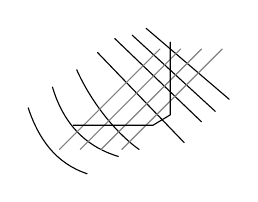
\begin{tikzpicture}[scale=.44,line cap=round]
\draw (0,.2)..controls (.3,-.7) and (.8,-1.4)..(1.7,-1.7);
\draw (.7,.8)..controls (1,-.2) and (1.6,-.9)..(2.6,-1.2);
\draw (1.4,1.3)..controls (1.8,.4) and (2.5,-.5)..(3.2,-1);
\draw (2,1.8)--(4.5,-.8); \draw (2.5,2.2)--(5,-.2);
\draw (3,2.3)--(5.4,.1); \draw (3.4,2.5)--(5.8,.45);
\foreach \x in {0,.6,1.2,1.8}{\draw[gray,thin] (\x+.9,-1)--(\x+3.8,1.9);}
\draw (1.3,-.3)--(3.6,-.3)--(4.1,0)--(4.1,2.1);
\end{tikzpicture}}
\[
\begin{aligned}
H^*(K(G_a,n),G_a)&=\text{\unsure{Cl.|\ensuremath{\mathscr A\cdot}} les op}\\
H^*(\mathbb Z[K(G_a,n)],G_a)&
\end{aligned}
\]
% slanted
Illusie $\unsure{X\in\text{cat }D,(T)|X\text{ cat }D,(T)|X\in\mathrm{ob}\,D_{\bullet}(T)}$ cat derivée des fais simpl\qquad $F$ objet abelien
\diagram{\begin{tikzcd}[ampersand replacement=\&,column sep=small]
\&H^*(X,F^{\unsure{*|\prime}})=[X,K(F,n)]\\
H^j(X_i,F)\arrow[ur,Rightarrow]\& X'\arrow[r]\arrow[d] \& K(F,n)\\
\&X
\end{tikzcd}}
\margin{Epstein L. Operations in homological algebra\par Invent. Math. 1 (1966)}

Illusie p 69\qquad 3.2.1.19 -- 3.2.1.18
\[
\begin{aligned}
&\operatorname{Ext}^{p}(N(X),F)=\lim_{\substack{X'\to X\\\mathrm{qis}\\\text{fibrant}}}[X',K(F,p)]\\
&\text{dit }''\, H^p(X,F)
\end{aligned}
\]
\[
\operatorname{Ext}^p(N(-),F)\longrightarrow\operatorname{Ext}^q(N(\ ),G)
\]
% slanted
Op coh de type $(F,p,G,q)$ sont class par $H^q(K(F,p),G)$
\margin{$\unsure{Z|z|\mathbb Z}X\xrightarrow{f}K(A,q$}

\[
H^n(K(G_a,m),G_a)=R^n\operatorname{Sym}(\mathbb F_p[m])
=\text{dual de }L^n\Gamma\,\deleted{\unsure{\mathrm{Hom}|\mathrm{Sym}}}(\mathbb F_p[m])
\]
\uline{Theoreme} : Soit $\mathscr A$ l'algebre sur $\mathbb F_p$ eng par $P^i$\qquad
$\deg P^i=2i(p-1)$\qquad $i\geq0$ sat aux relations d'Adem (mais non à $P^0=1$).
\[
H^*(K(\deleted{G_a}\mathcal O,m),\deleted{G_a}\mathcal O)
\]
est l'alg anticomm libre engendrée par les monomes admissibles de $\mathscr A$ d'exces $<n$.
\margin{$H^*(K(\mathbb F_{p^h},n),\mathbb F_{p^h})$}

\uline{Dém} : Comme dans le cas classique, il suffit de calculer $H^*(K(G_a,1),G_a)$ et de grimper en utilisant le th de Borel et la suite sp de Leray associée à
\diagram{\begin{tikzcd}[ampersand replacement=\&]
K(G_a,n-1)\arrow[r]\& *\arrow[d]\\
\&K(G_a,n)
\end{tikzcd}}
$\downarrow$\quad Lazard : Coh de l'analyseur classique dans ``Lois de groupes formels et analyseurs'' Ann ENS

\margin{$R$ anneau de car $p\unsure{>|{\geq}}0$\par $H^*(K(R,n),R)=$ Alg anticomm libre /$R$ eng par $\operatorname{Hom}_{\rm Ab}(R,R)$-module libre eng par les monomes admissibles $f\in\operatorname{Hom}(R,R)$}
\margin{$\oplus\ P^If\iota_n$\par $\underset{\rotatebox{90}{$\in$}\,x}{H^*(X,\mathcal O)}\longrightarrow\underset{P^Ix}{H^*(X,\mathcal O)}$\par $\mathrm{Hom}$}
\diagram{\begin{tikzcd}[ampersand replacement=\&,row sep=small]
G_a^3\&G_a\times G_a\&G_a\\
\&\&\deleted{\operatorname{Sym}\mathbb F_p}\\
k[x,y,z]\&k[x,y]\arrow[l]\&k[x]\arrow[l]
\end{tikzcd}}
\[
\begin{aligned}
\iota_1&\in H^1(K(G_a,1),G_a)\\
\text{Witt}\ \longleftarrow\ \beta&\in H^2(K(G_a,1),G_a)\\
0\to G_a\to W_2&\to G_a\to0\\
0\to\mathbb Z/p\to\mathbb Z/p^2&\to\mathbb Z/p\to0
\end{aligned}
\]
On se ramène au calcul de
\diagram{\begin{tikzcd}[ampersand replacement=\&]
\&H^*(K(\mathbb F_{p^h};1),\mathbb F_{p^h})\\
x\in H^n(K(\mathcal O,m),\mathcal O)\arrow[ur]\& {}\\
K(\mathcal O,m)\arrow[r]\&K(\mathcal O,n)\\
K(R,m)\arrow[r]\&K(R,n)\qquad\forall R/\mathbb F_p
\end{tikzcd}}
\noindent\rule{.8\linewidth}{.3pt}

représenté par des polynomes de deg $<p^h$ en chaque var
\[
x\in H^*(K(\mathcal O,n),\mathcal O)_h\xrightarrow{\text{injective}}H^*(K(\mathbb F_{p^h},n),\mathbb F_{p^h})
\]
% archive sheet number: 376
\scanpage{375}
\uuline{Calcul des $\operatorname{Ext}^i(G_a,G_a)$}

\uline{Prop} : Le $k[F]$-module $\operatorname{Ext}^i(G_a,G_a)$ (pour l'action de $\operatorname{Hom}(G_a,G_a)$ à droite) est de $F$ torsion $(i>\deleted{\unsure{0}}1)$.

\uline{Cor} : (\unsure{Milne|Mhre}) $G_a^{\rm perf}=$ restriction de $G_a$ au site parfait /$k$
\[
\begin{aligned}
G_a^{\rm perf}&=\lim_{\substack{\longleftarrow\\ F}}G_a\\
\operatorname{Ext}^i(G_a^{\rm perf},G_a^{\rm perf})&=0\qquad i>1.
\end{aligned}
\]
$\searrow$\quad\uline{Dém} : On considere la suite spectrale du coefficient universel
\[
\forall\ \text{fais simpl }X:\ E_2^{i,j}=\operatorname{Ext}^i_{\mathbb F_p}(\underline H_j(X),F)\Longrightarrow \mathbb H^{i+j}(X,F)
\]
En fait on va travailler dans la catégorie des fais de $\mathbb F_p$-modules

On travaille mod $F$ (au sens mod $\mathcal C$)
\[
\begin{aligned}
\operatorname{Hom}(G_a,G_a)&=k[F]\\
\operatorname{Ext}^1(G_a,G_a)&=0
\end{aligned}
\]
\margin{$\deleted{E^{*,j}}=\deleted{0}$\par $\deleted{j<n}$}

Dem par récurrence : On va considerer la s. spectrale précedente avec $X=K(G_a,n)$\qquad $\deleted{\operatorname{Ext}^i}$\quad $n$ grand.
\[
\begin{aligned}
E\qquad&\operatorname{Ext}^i(H_j(K(G_a,n)),G_a)\Longrightarrow H^*(K(G_a,n),G_a)\\
E_2^{i,n}&=\operatorname{Ext}^i(H_n(K(G_a,n)\ G_a)\\
&\underset{\operatorname{Ext}^i(G_a,G_a)}{\shortparallel}
\end{aligned}
\]
\figure{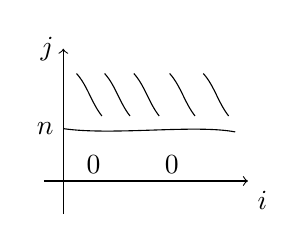
\begin{tikzpicture}[scale=.70]
\draw[->] (-.35,0)--(3.35,0) node[below right] {$i$};
\draw[->] (0,-.6)--(0,2.4) node[left] {$j$};
\draw (0,.95) node[left] {$n$}..controls (.9,.82) and (2.4,1.03)..(3.12,.89);
\node at (.55,.29) {$0$};\node at (1.97,.29) {$0$};
\foreach \x in {.24,.75,1.28,1.93,2.54}{\draw (\x,1.95)..controls (\x+.2,1.73) and (\x+.27,1.42)..(\x+.46,1.18);}
\end{tikzpicture}}
\[
\underline H_j(K(G_a,n)=\bigoplus G_a\qquad G_a\xrightarrow{p=0}G_a
\]
% archive sheet number: 377
\scanpage{376}
\[
\operatorname{Ext}^i(H_j(K(G_a,n),G_a)\Longrightarrow\mathbb H^{i+j}(K(G_a,n),G_a)
\]
On raisonne par récurrence, mod $F$
\diagram{\resizebox{\linewidth}{!}{\begin{tikzcd}[ampersand replacement=\&,column sep=small]
\operatorname{Ext}^i(H_n(\deleted{K(G_a,n)},G_a)\arrow[r]
\&H^{n+i}(K(G_a,n),G_a)\arrow[r]
\&\operatorname{Hom}(H_{n+i}(K(G_a,n)),G_a)\arrow[r]
\&\operatorname{Ext}^{i+1}(\unsure{G_a'|G_a},G_a')\arrow[r,"\partial"]\arrow[d]
\&H^{n+i+1}(K(G_a,n),G_a)\arrow[d,leftrightarrow]\\
0\arrow[ur]\&{}\&\underset{\bigoplus\operatorname{Hom}(G_a,G_a)}{\shortparallel}
\&\underset{\underset{0}{\shortparallel}}{\operatorname{Ext}^{i+1}(\mathbb F_{p^h},\mathbb F_{p^h})}\arrow[r,"\partial"]
\&H^{n+i+1}(K(\mathbb F_{p^h},n),\mathbb F_{p^h})
\end{tikzcd}}}

\uline{Lemme 1} le edge homomorphism $\partial$ est nul.

\uline{lemme 2}\qquad $x$ un generateur de
\[
\begin{aligned}
H^{n+i}(K(G_a,n),G_a)&\longrightarrow\operatorname{Hom}(H_{n+i}(K(G_a,n)),G_a)\\
P^I\iota_n&\hspace{4em}\shortparallel\\
\beta\underbrace{P^{i_1}\beta\cdots P^{i_r}}_{\text{longueur }r+s}\iota_n
 &\qquad\operatorname{Hom}(G_a\otimes H_{n+i}(K(\mathbb F_p,n)),G_a)\\
&\hspace{4em}\shortparallel\\
&\big(H^{n+i}(K(\mathbb F_p,n),\mathbb F_p)\otimes\operatorname{Hom}(G_a,G_a)\\
P^d\iota_n&\longrightarrow P^d\iota_n\otimes F
\end{aligned}
\]
Dém\qquad \unsure{on} le demontre pour $P^0\iota_n$

\medskip\centerline{\rule{1.0cm}{.3pt}}
\[
\begin{aligned}
\operatorname{Ext}_{\mathbb F_p}^*(G_a,G_a)\qquad
\operatorname{Ext}^{2i+1}(G_a,G_a)&=0\qquad \forall i\quad i>0\\
\operatorname{Ext}^{2i}(G_a,G_a)&=\frac{k[F]}{(F^d)}\qquad d=v_p(i).
\end{aligned}
\]
\diagram{\begin{tikzcd}[ampersand replacement=\&,column sep=small,row sep=tiny]
\mathscr A\arrow[r]\& A\&\mathscr A\arrow[r]\&\mathscr A\otimes\mathscr A\\
P^i\arrow[r]\&P^i\&P^i\arrow[r]\&\displaystyle\sum_{j+k=i}P^j\otimes P^k\\
P^0\arrow[r]\&1\&{}\&{}
\end{tikzcd}}
\medskip\centerline{\rule{1.5cm}{.3pt}}
\[
\operatorname{Ext}^i(\mathbb Z^{\unsure{j|*}}K(G_a,n),G_a)\Longrightarrow\operatorname{Ext}^{i+j}(G_a,G_a)
\]
\[
K(\mathbb Z)=K(\mathbb Z,m)\qquad n\ \text{grand}
\]
\diagram{\resizebox{\linewidth}{!}{\begin{tikzcd}[ampersand replacement=\&,column sep=small]
Z^iK(G_a,n)\arrow[r,shift left=.6ex]\arrow[r,shift right=.6ex] \& \cdots\arrow[r,shift left=1ex]\arrow[r]\arrow[r,shift right=1ex]
\&ZZK(G_a,n)\arrow[r,shift left=.65ex]\arrow[r,shift right=.65ex]\&ZK(G_a,n)
\end{tikzcd}}}
\[
Z[Z^{j-1}K(G_a,n)]\sim Z[K(Z)\wedge K(Z)\wedge\cdots\wedge K(G_a,n)]
\]
\diagram{\begin{tikzcd}[ampersand replacement=\&,column sep=small,row sep=small]
E_1\quad\ldots\& A^{\otimes2}\otimes\mathscr A \& A\otimes\mathscr A\arrow[l,shift left=1ex]\arrow[l]\arrow[l,shift right=1ex]\&\mathscr A\arrow[l,shift left=.6ex]\arrow[l,shift right=.6ex]\\
\text{Dualement}\quad\ldots\& A_*^{\otimes2}\otimes\mathscr A_*\arrow[r,shift left=1ex]\arrow[r]\arrow[r,shift right=1ex]\& A_*\otimes\mathscr A_*\arrow[r,shift left=.6ex]\arrow[r,shift right=.6ex]\&\mathscr A_*
\end{tikzcd}}
\[
\begin{aligned}
E_2^{i,j}&=\widetilde H^{\unsure{i|*}}(K(Z)^{\wedge j-1}\wedge K(G_a),G_a)
\overset{\text{Kunneth}}{\sim}\widetilde H^*(K(Z))^{\otimes j-1}\otimes\widetilde H^*(K(G_a),G_a)\\
H^*(K(\mathbb F_p),\mathbb F_p)&= A\\
H^*(K(G_a),G_a)&=\mathscr A
\end{aligned}
\]
\[
E^2=\operatorname{Tor}^{A_*}(\mathscr A_*,\mathbb F_p)\Longrightarrow \unsure{E^2|t^2|k^2}\ \text{par Koszul}
\]
% archive sheet number: 378
